%%%%%%%%%%%%%%%%%%%%%%%%%%%%%%%%%%%%%%%%%%%%%%
%% Copyright 2020 Andrew Cuccinello
%%
%% Licensed under the Apache License, Version 2.0 (the "License");
%% you may not use this file except in compliance with the License.
%% You may obtain a copy of the License at
%%
%%     http://www.apache.org/licenses/LICENSE-2.0
%%
%% Unless required by applicable law or agreed to in writing, software
%% distributed under the License is distributed on an "AS IS" BASIS,
%% WITHOUT WARRANTIES OR CONDITIONS OF ANY KIND, either express or implied.
%% See the License for the specific language governing permissions and
%% limitations under the License.

\documentclass{article}
\usepackage{fullpage}
\usepackage{graphicx}
\usepackage{hyperref}
\hypersetup{
    colorlinks=true,
    linkcolor=blue,
    filecolor=magenta,
    urlcolor=cyan,
}

\title{%
    PDFoundry \\
    \large User Manual}
\date{}
\author{}

\setcounter{tocdepth}{2}
\begin{document}
    \begin{figure}[t]
        \centering
        
\includegraphics[width=0.5\textwidth]{images/logo.png}
    \end{figure}
    \maketitle

    If you're seeing this - it means your system now supports \textit{PDFoundry}, a FoundryVTT PDF reader. Likely, you just updated and are confused about what this is - so this guide goes over the features available and their use. This user manual also functions as a demo, and you can always access it through the \textbf{settings menu}, if you wish to do so later.

    \tableofcontents

    \section{How to Use}
    One of the reasons \textit{PDFoundry} requires integration with a system is it's tight integration with the core system. You do most things in PDFoundry through \textit{items}. Just like you would normally create a weapon or armor, you can create a PDF. You'll have the option to setup what file on the server this PDF points to (or upload one), as well as a few other options.

    \subsection{The Basic Steps - Adding a PDF}
    This section outlines basic steps to adding a new PDF and outlines what each PDF setting does.

    \begin{description}
        \item [Step 1] Open the \textbf{Items Directory} and click \textbf{Create Item}. Enter a \textbf{Name}, in Figure~\ref{new-item} I've chosen to add the core rule book for the RPG \textit{Lancer} (\href{https://massif-press.itch.io/corebook-pdf-free}{available for free online!}), so I'll name this one \textit{Lancer Core Rulebook}. Select \textbf{PDFoundry\_PDF} for the \textbf{Type} drop-down, then click \textbf{Create Item}.

        \begin{figure}[h]
            \centering
            \begin{minipage}[t]{0.45\textwidth}
                \centering
                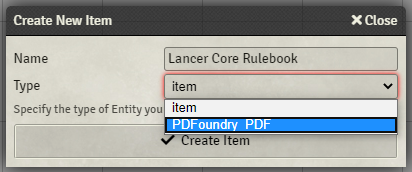
\includegraphics[width=\textwidth]{images/new-item.png}
                \caption{A created item in the \textbf{Item Directory}}
                \label{new-item}
            \end{minipage}
            \hfill
            \begin{minipage}[t]{0.45\textwidth}
                \centering
                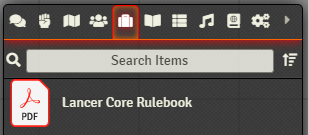
\includegraphics[width=\textwidth]{images/new-item-created.png}
                \caption{The \textbf{New Item} dialog}

                \label{new-item-created}
            \end{minipage}
        \end{figure}

        \item [Step 2] After you've hit \textbf{Create Item} the \textbf{PDF Sheet} should open automatically and look something like Figure~\ref{new-item-sheet}. You'll also see the PDF get placed in your item directory, as in Figure~\ref{new-item-created}. There are a bunch of fields on the \textbf{PDF Sheet}, \textit{PDF Name} is already filled in for us (but we can change it if we want!). Next let's fill in all the fields.

        \begin{figure}[h]
            \centering
            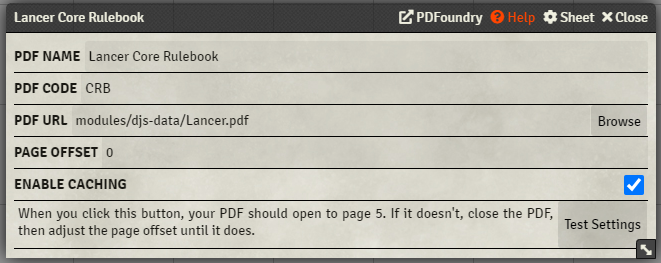
\includegraphics[width=1\textwidth]{images/new-item-sheet.png}
            \caption{The \textbf{PDF Sheet}}
            \label{new-item-sheet}
        \end{figure}

        \item [\textit{PDF Code}] This is a short (usually five characters or less) identifier you will use in most systems. It is up to the individual system exactly what you will use, so you should look at an additional information provided by the system.

        \item [\textit{PDF URL}] This is the path to the PDF on your server. The browse button will allow you to select or upload a PDF. Mine is my module I made to share data between my worlds, but you can put it wherever you want.

        \item [\textit{Page Offset}] Some PDF files have extra pages before the first page, such as a title or unnumbered index page. You can use this to synchronize the PDF page to the book page. The Lancer book doesn't need an offset, so it's zero here.

        \item [\textit{Enable Caching}] Tick this box to enable caching for this PDF. That is, when a user opens the PDF, should the PDF be preserved locally on the user's computer to allow subsequent opens without having to fetch it from the server. \underline{To preload PDFs, this must be enabled.}

        \item [Step 3] Now that we've entered all our settings in, we can use the \textbf{Test Settings} button to open the PDF to page 5. We want the PDF to open to page 5 of the book, so that when we have a page reference it opens to the correct page.

    \end{description}

    That's it, we've added a new PDF!

    \subsection{Context Menu Options}
    We saw the PDF appear in the \textbf{Items Directory} earlier, when we created a \textbf{new item}. Figure~\ref{new-item-context} shows the context menu options for PDF items. You can open the context menu with \textbf{right click}. There are a bunch of options that you as the GM can see, while players will only be able to see the \textbf{Open PDF} and \textbf{View Item Artwork} options.

    \begin{figure}[h]
        \centering
        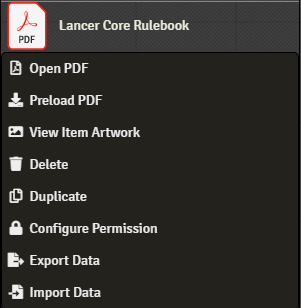
\includegraphics[width=0.5\textwidth]{images/new-item-context.png}
        \caption{The PDF \textbf{Context Menu}}
        \label{new-item-context}
    \end{figure}

    \begin{description}

        \item [Open PDF] (All Users) This one should be mostly self explanatory. It won't show up unless the \textbf{PDF URL} has been fully configured. Clicking on it opens the PDF to the very first page.

        \item [Preload PDF] (GM Only) Click on it will immediately cache the PDF on all \underline{connected} users' computers. This may be advantageous in cases where you expect to often use a single large book and don't want users downloading the PDF files to interrupt other goings on in the game.

        \item [View Item Artwork] (All Users) For now this only shows the PDF thumbnail. Thumbnail support based on the linked file is planned.

        \item [Delete] (GM Only) This will irrevocably delete the link to the PDF file. The PDF file itself is not affected.

        \item [Duplicate] (GM Only) This will duplicate the link to the PDF file by creating a copy of the item.

        \item [Configure Permission] (GM Only) This will allow you to grant visibility of the PDF to players, either individually or all players. The permissions work much like permissions for other things in Foundry; however, if the PDF is visible to the player at all (that is if their permissions are anything \underline{except 'None'}) the user will be able to right click on the PDF to open it, and any other links to the PDF will function correctly (such as 'open to page' links added by a system).

        \item [Export Data] This will allow you to export a file that can later be used with the \textbf{Import Data} option.

        \item [Import Data] This will allow you to import the settings for a PDF (Name, Code, URL, etc) from a file created with the \textbf{Export Data} option.

    \end{description}

    \section{Settings Configuration}
    There is only one setting at present for PDFoundry. It is located with your system settings in the \textbf{Game Settings} $>$ \textbf{Configure Settings} $>$ \textbf{System Settings} menu.

    \begin{description}
        \item \subsection{PDF Cache Size} This allows individual users to set how much hard drive space should be allowed to be taken up by the PDF cache. When this amount is exceeded, PDFoundry will prune existing cached PDF files in reverse order of most recently accessed. That is to say, PDF files will be removed from the cache starting with the file that has least recently accessed.
    \end{description}

\end{document}